\documentclass[tikz,fontsize=8pt]{standalone}
\usepackage{fourier}
\usetikzlibrary{arrows.meta}
\usetikzlibrary{calc}
\tikzset{>=latex}
\definecolor{bookblue}{RGB}{0,173,239}
\definecolor{bookpink}{RGB}{236,0,140}
\definecolor{bookgreen}{RGB}{50,200,0}
\definecolor{bookbluearea}{RGB}{204,239,252}
\tikzstyle{blueline}=[draw=bookblue,line width=0.2mm]
\tikzstyle{pinkline}=[draw=bookpink,line width=0.2mm]
\tikzstyle{greenline}=[draw=bookgreen,line width=0.2mm]
\tikzstyle{blackline}=[draw=black,line width=0.2mm]
\tikzstyle{bluearea}=[fill=bookbluearea]

\usepackage{scrextend}
\changefontsizes[8pt]{8pt}
\usepackage[utf8]{inputenc}
\usetikzlibrary{decorations.pathreplacing}
\begin{document}
  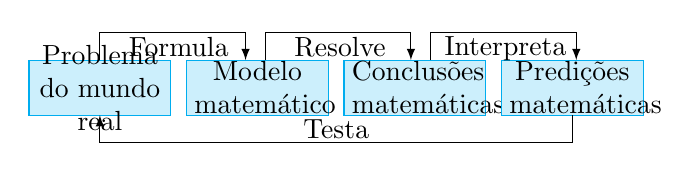
\begin{tikzpicture}
  \draw [fill=bookbluearea,draw=bookblue](0,0) rectangle (1.8,0.7) node[pos=.5,text width=1.6cm,align=center]{Problema do mundo real};
  \draw [fill=bookbluearea,draw=bookblue](2,0) rectangle +(1.8,0.7) node[pos=.5,text width=1.6cm,align=center]{Modelo matemático};
  \draw [fill=bookbluearea,draw=bookblue](4,0) rectangle +(1.8,0.7) node[pos=.5,text width=1.6cm,align=center]{Conclusões matemáticas};
  \draw [fill=bookbluearea,draw=bookblue](6,0) rectangle +(1.8,0.7) node[pos=.5,text width=1.6cm,align=center]{Predições matemáticas};
  \path[->,draw=black](0.9,0.7)--+(0,0.35)--+(1.85,0.35)--+(1.85,0);
  \path[->,draw=black](3,0.7)--+(0,0.35)--+(1.85,0.35)--+(1.85,0);
  \path[->,draw=black](5.1,0.7)--+(0,0.35)--+(1.85,0.35)--+(1.85,0);
  \path[->,draw=black](6.9,0)--+(0,-0.35)--+(-6,-0.35)--+(-6,0);
  
  \node at (1.9,0.87) {Formula};
  \node at (3.95,0.87) {Resolve};
  \node at (6.05,0.84) {Interpreta};
  \node at (3.9,-0.18) {Testa};
  \end{tikzpicture}
\end{document}